%packages a utilizar:
\documentclass{report}
\usepackage[T1]{fontenc}     % Fontes T1
\usepackage[utf8]{inputenc}  % Input UTF8
\usepackage[top=3cm,bottom=3cm,left=3cm,right=2.5cm,asymmetric]{geometry} %fronteiras
%\usepackage[nottoc]{tocbibind}
\usepackage[table]{xcolor} %Colorir tabelas
\usepackage[backend=biber, style=ieee]{biblatex} %bibliografia
\usepackage{csquotes}  % referências
\usepackage[portuguese]{babel} %Usar língua portuguesa
\usepackage{blindtext} 
\usepackage[printonlyused]{acronym}  %Acrónimos
\usepackage{hyperref}  %Autoref no índice
\usepackage{graphicx}  %Usar imagens
\usepackage{titling}
\usepackage{multicol} %multicoluna de texto
\usepackage{adjustbox}
\renewcommand{\figurename}{Fig.} 
\renewcommand{\tablename}{Tabela} 
\usepackage[font=small,tableposition=top]{caption} 
\usepackage[font=small]{subcaption}
\usepackage{xcolor} %cor nos textos
\usepackage{amsmath} %matematica
\usepackage{amssymb} %simbolos matematicos
\graphicspath{ {./images/} } %directorio das imagens
\usepackage{fancyhdr}
\usepackage{authblk}
\usepackage{float} %Posicionamento exacto das figuras no texto
\usepackage{url}   %referencias URL
\usepackage{blindtext}
\def\UrlBreaks{\do\/\do-} %não cortar referencias

\usepackage{indentfirst} %Garantir avanço do primeiro parágrafo
\hypersetup{pdfborder=0 0 0} %Remover a caixa vermelha das referências
\usepackage{chngcntr} %Numeração contínua das figuras
\counterwithout{figure}{chapter} %Numeração contínua de figuras
\counterwithout{table}{chapter} %Numeração contínnua de tabelas
\setlength{\parskip}{0.2cm} %Aumento de espaçamento entre parágrafos

\usepackage{hyperref}

 
\begin{document}	
	%Definições do Relatório

%Dados Gerais:
\def\titulo{Projecto Final: \\ Máquina de Lavagem de Roupa}
\def\data{Junho de 2022}
\def\versao{Ver.: 1.13}
\def\departamento{Departamento de Electrónica Telecomunicações e Informática}
\def\empresa{Universidade de Aveiro}
\def\logotipo{logotipo_ua.png}

%Dados dos Autores:
%primeiro autor:
\def\pautor{João Pedro Nunes Vieira} 
\def\numpautor{Nº Mec.:  50458}
\def\contactopautor{joaopvieira@ua.pt}
%segundo autor:
\def\sautor{Leandro Roque Costa} 
\def\numsautor{Nº Mec.: 110326}
\def\contactosautor{lrc@ua.pt}
%
\def\autores{\pautor \\ \sautor}

	%Capa do Relatório:
\begin{titlepage} 
	\begin{center}
	\includegraphics[scale=0.50]{\logotipo}
	\line(1,0){350} \\ 
		\vspace*{2mm}
	{\Large \uc} \\
		\vspace*{2mm} 	
	{\Huge \titulo} \\
		\vspace*{2mm}
	\line(1,0){350} \\ 
		\vspace*{2mm}
	{\Large \empresa} \\
		\vspace*{20mm}
	{\Large \autores} \\ 
		\vspace*{\fill}
	\end{center}

	\begin{flushright} 
		{\large \departamento} \\ 
		{\versao} 
	\end{flushright}

\end{titlepage}

	%Página de Título:
\predate{\begin{flushright}\small}
\postdate{\par\end{flushright}}

\title{ 
	{\huge\textbf{\titulo} } \\ 
	{\large \departamento\\ \empresa} }

\author{

    \begin{tabular}{l}
        \pautor, \numpautor\hfil \\
        \contactopautor
    \end{tabular}
    \and
    \begin{tabular}{l}
        \sautor, \numsautor\hfil \\
        \contactosautor
    \end{tabular}
    \and
    \begin{tabular}{l}
        \tautor, \numtautor\hfil \\
        \contactotautor
    \end{tabular}
    \and
    \begin{tabular}{l}
        \qautor, \numqautor\hfil \\
        \contactoqautor
    \end{tabular}
}




\date{\vspace{\fill}{\data}} 
\maketitle
	\begin{abstract}

O presente relatório aborda a comunicação entre aplicações seguindo um modelo Cliente-Servidor, usando conceitos abordados no decorrer da Unidade Curricular de Laboratórios de Informática, nomeadamente programação de sockets TCP, Criptografia, Documentação JSON, programação em Python, etc... \\
Este trabalho é relevante pois com o avanço tecnológico actual, a aprendizagem dos conceitos anteriormente referidos torna-se imperativa para os estudantes de cursos ligados à tecnologia de informação.\\
O projecto foi realizado por duas pessoas, tendo como objectivo o desenvolvimento das capacidades de trabalho em grupo, desenvolvimento e estruturação de código, realização de testes funcionais e planeamento através da plataforma \textbf{code.ua.pt}. \\
Foi possível implementar com sucesso um modelo de comunicação entre aplicações Cliente-Servidor em gênero "Jogo High-Low" com funcionalidade de segurança(encriptação) de forma simples, prática e eficaz, conseguindo-se corrigir todos os erros encontrados.

\end{abstract}
	%Agradecimentos:
\renewcommand{\abstractname}{Agradecimentos}
\begin{abstract}
"Em construção"
%se for necessário usar: Colegas e/ou pessoas que nos ajudaram. 
\end{abstract}
	
%########################################################	
%ÍNDICE:
	\renewcommand{\contentsname}{Índice}
	\tableofcontents
	\listoffigures
	\pagenumbering{roman}

%########################################################	
%HEADERS & FOOTERS:
\pagestyle{fancy}
\fancyhf{}
\rhead{\titulo}
\lhead{Introdução}
\cfoot{\thepage}

%########################################################	
%########################################################	
%CAPÍTULO 1: Introdução

\chapter{Introdução}
\label{chap.introdução}
\pagenumbering{arabic}
\begin{multicols}{2}
A montagem e diagnóstico de computadores pessoais é um tema cada vez mais relevante nesta nova era digital. Segundo o Instituito Nacional de Estatisticas no ano 2017, cerca de 71.5~\% dos agregados domésticos privados tem um computador pessoal e no presente ano 2020, o número de utilizadores de novas tecnologias duplicou em percentagem por motivos educativos, devido à pandemia COVID-19.  Assim, focando nos em Computadores Desktop (ou fixos), seria benéfico compactar num único local todo o conhecimento necessário evitando avarias e desinformação sendo que existem dois lados a considerar no que toca à aprendizagem sobre este assunto:\\
Existem diversos livros volumosos de autores legítimos, contudo muitos de nós não pretende ler uma redação inteira sobre o assunto que muitas vezes contempla pontos complexos, os quais têm pouco interesse para quem apenas quer montar o seu computador pessoal sem grandes complicações.\\
Por outro lado vivemos numa era digital, e existe uma enorme quantidade de informação difundida por diversas plataformas online (Forums, Youtube, Blogs, etc…). Muitas vezes esta difusão resulta em informação distorcida e desinformação, devido a interpretações erradas, pesquisa limitada, opiniões não fundamentadas ou influenciadas, especulação ou até interesses maiores.\\
Esta é a realidade que vivemos, a qual temos por objetivo contrariar de modo a fornecer a quem tenha acesso a este trabalho, toda informação necessária para a montagem do seu PC fixo e com tal, necessitamos de conhecer as peças no seu interior. 
\end{multicols}

\section{Introdução Análoga: E se um PC fosse uma Pessoa?}
\label{sec.analoga}
[ Tal como uma pessoa um computador tem "orgãos" (ie. componentes internos) que o fazem funcionar correctamente. Estes componentes são designados de \textbf{"Hardware"} e a cada peça é atribuida uma função principal no funcionamento correcto da máquina.]
Pensando num PC como se fosse um ser humano, podemos admitir que o seu cerebro é composto por três comonentes internos distintos. O \ac{cpu}, tem como função realizar intruções de programas, realizar operações matemáricas (aritmética), lógica e gerir a entrada e saida de dados, contudo não armazena informação. Nesta analogia\footnotemark[1], pensando em \textbf{\textsl{informação}} como \textbf{\textsl{"memórias humanas"}}, a função de armazenamento é atribuida a dois componentes distindos: a \ac{ram} e \ac{uad}. A \ac{ram} é o local onde se executa a leitura e escrita de informação volátil (ie.: informação acessivel mas não gravada), que pode ser análoga a memórias humanas de curto prazo, as quais não guardamos e recordamos num futuro a longo e médio prazo. Para gravar estas informações de forma a serem acessadas no futuro, é usado uma (ou mais) \acf{uad}, da qual existem diversos tipos, que iremos falar mais à frente no Capítulo 8. \\
Sendo o \textbf{\textsl{"cérebro do computador"}} um conjunto de componentes distintos, estes têm que ser conectados entre sí, através de um \textbf{"tronco"} e \textbf{"sistema nervoso"}. Num computador podemos considerar como "tronco" a \textbf{Motherboard}, pois é nesta que todos os componentes do compotador são conectados físicamente e controlados pelo sistema nervoso do equipamento, que neste caso iremos considerar como o \textbf{Chipset} pois é imbutido e ligado na Motherboard e é o responsável pela gestão do fluxo de dados entre o \ac{cpu}, memória e periféricos. \\
Ora, um tronco e uma cabeça só, não faz uma pessoa. Necessitamos de pernas e braços para andar, comer, trabalhar, vier, etc... Num computador esta função é desempenhada pela \ac{gpu}, que é um tipo de microprocessador especialmente desenhado para processar e apresentar gráficos (\textit{ie.: imagens}) ao utilizador. Podemos considerar a \ac{gpu} como as pernas e braços de uma pessoa pois sem esta não o equipamento funciona, mas não desempenha funções relevantes para o utilizador. Por outro lado uma \ac{gpu} não dedicada (\textit{ie.:"fraca"}) desempenha funções simples mas não consegue (na geralidade) desempenhar acções mais exigentes (\textit{exemplo.: renderização de gráficos}). Análogamente, quanto mais fortes os musculos das nossas pernas e braços, maior é a nossa capacidade actividade física. \\ 
O no corpo humano existem diversos orgão que dão vida e energia a uma pessoa como coração, pulmões, estomago etc... Nesta analogia, todos estes podem ser considerados como a \ac{psu}, do equipamento que fornece energia electrica e assim "vida" à máquina.
Para finalizar, necessitamos de um esqueleto para proteger os nossos orgão e mantermos tudo no seu lugar, que no caso de um PC é nada mais nada menos que a Caixa externa de PC que contem todos este componentes e é (geralmente) a primeiro compoennte do PC que vemos no nosso dia a a dia.

\footnote{Analogia: Relação de semelhanças entre objectos diferentes.}

%########################################################	
%########################################################	
%CAPÍTULO 2: Ferramentas e Cuidados Essenciais

\chapter{Ferramentas e Cuidados Essenciais}	
\label{chap.cuidados}
\lhead{Ferramentas e Cuidados Essenciais}
Para a assemblagem de um equipamento informático, são necessárias algumas ferramentas e cuidados gerais e essenciais a ter em conta, evitando assim avarias e mantendo o utilizador em segurança.
\section{Ferramentas}
\label{sec.ferramentas}
Existem diversas ferramentas para executar a abertura de um PC. A grande maioria delas depende do tipo de cabeça de parafusos existentes no interior do equipamento sendo as mais comuns as seguintes:

	\begin{figure}[h!]
		\centering
		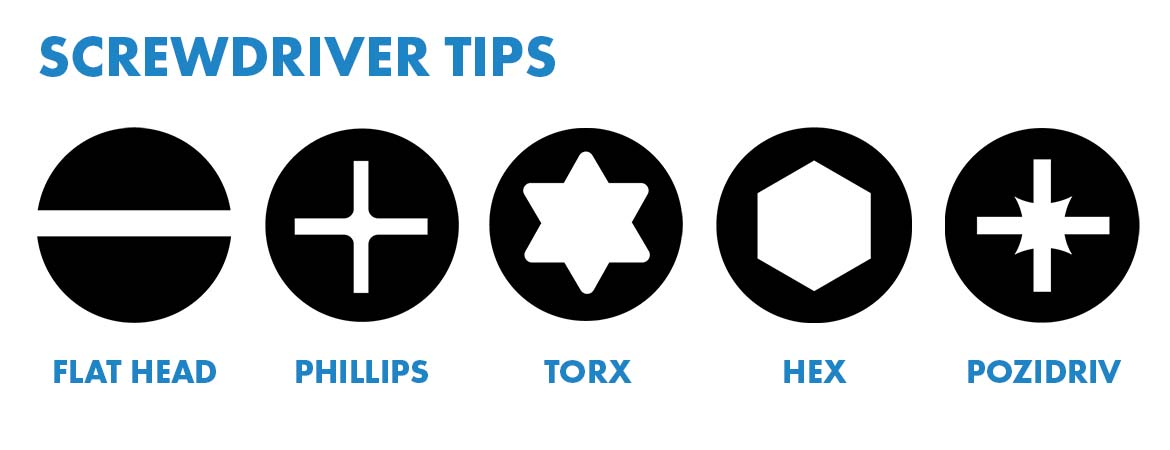
\includegraphics[width=15cm]{./chaves.jpeg}
		\caption{Diferentes tipos de cabeças de parafusos, \\ \textsl{imagens de www.heamar.co.uk}}
		\label{fig.cabeçasparafusos}
	\end{figure} 


\section{Cuidados Essenciais}
Existem alguns cuidados básicos que não devem ser ignorados ao tentar montar e/ou intervencionar o seu computador:

\begin{enumerate}
	\item \textbf{Desligar o computador da corrente elétrica antes de abrir ou intrevencionar:} Este passo, de extrema importancia por razões obvias, evita não só avaria dos componentes a serem intrevencionados como também mantem em segurança o utilizador (tecnico) durante a intrevenção.
	\item \textbf{Libertar a eletrecidade estática}: O uso de luvas ou pulseira anti-estática como referido anteiormente, permite a libertar a electricidade estática do nosso que pode ter sido acomulada através de diversos factores. Ao executar este passo, evita que ao manusear os componentes do seu equipamento os avarie acidentalmente, pois são muito sensíveis a choques electroestáticos. Em caso de não ter uma das ferramentas referidas, pode tocar numa peça de metal que não esteja directamente ligada ao seu PC.
	\item \textbf{Organizar o espaço de trabalho:} A organização do espaço de trabalho é essencial para manter todo o processo livre de complicações ou percalços. Assim, deve ter uma bancada de trabalho limpa e establizada, ferramentas e componentes organizados e parafusos organizados e númerados por ordem. \\ 
	\textsl{\textbf{Dica:} Se for necessário, faça um desenho com a localização e a ligação dos componentes}.
	\item \textbf{Nunca deixar cabos soltos por cima de ventoinhas:} evitando assim, barulho ao colocar o equipamento em funcionamento e (mais importante) danificar o cabo ou quebrar as pás da ventoinha em questão. 
	\item \textbf{Nunca forçar o encaixe dos componentes:} \textit{"Se não vai a bem, vai a mal"}. Esta é uma situação muito comum e perigosa, sendo que os encaixes de componentes são suaves e não devem ser forçados, sendo a única excepção á regra o encaixe de Slot da Memória RAM que por vezes necessita um pouco mais de força (\textbf{mas não muita!}), para que o encaixe se execute. 
\end{enumerate}

\section{Limpeza}
No que toca á limpeza da máquina também há algumas recomendações ,tais como:

\begin{enumerate}
	\item \textbf{Limpeza periódica:} Uma vez que o pc ao longo do tempo irá acumular grande quantidade de pó, cotão e desgaste na massa térmica, é recomendado executar uma limpeza interna de cotão de 6 em 6 meses e troca de massa térmica no máximo de 2 em 2 anos.
	\item \textbf{Produtos de Limpeza:} Quando for necessária a aplicação de produtos de limpeza, é importante evitar o uso de compostos com água,uma vez que contém sais condutores de eletricidade. Existem líquidos específicos, como o álcool isopropílico (líquido de alta volatiliade, evaporando com facilidade), que não tem água na sua composição tornando-os adequados para limpar componentes electrónicos.
\end{enumerate}

%########################################################	
%########################################################	
%CAPÍTULO 3: MOTHERBOARD
\chapter{Motherboard}
\lhead{Motherboard}
\label{chap.motherboard}
Como referimos na \textbf{Introdução Análoga} \ref{sec.analoga}, a motherboard (também conhecida como “placa mãe”), é um componente importante que conecta todo o hardware do nosso equipamento. Assim a escolha de uma motherboard não deve ser menosprezada face à escolha do CPU, GPU, RAM ou até SSD. É correto admitir que estes dois componentes são muitas vezes mais priorizados pois são eles que (essencialmente), permitem ao equipamento ter maior performance e versatilidade para executar programas ou aplicações instaláveis. \\
\\ \textbf{Muitas vezes, e por ignorância ou preguiça, executamos uma das seguintes linhas de pensamento:}
\begin{itemize}
\item A motherboard mais barata é a melhor porque só serve para ligar tudo.
\item A melhor a motherboard é a mais cara.
\end{itemize}
Ambas estas frases estão erradas. Para escolher uma mothebroard temos que olhar para as características que necessitamos ou desejamos no nosso futuro computador e avaliar qual a melhor escolha mediante o que pretendemos obter e preço que pretendemos pagar.
 A escolha de uma motherboard é extremamente importante, não só porque necessitamos de uma motherboard confiável de modo a evitar avarias, mas também porque é ela que delimita o número de portas I/O disponíveis, o tamanho que o equipamento futuramente terá, o CPU Socket e modelos de processadores que podem ser montados e o chipset que determina se há possibilidade de overclock, que componentes são compatíveis e quantidades dos mesmos aceites como: tipo de RAM e respetivas velocidades, voltagens e capacidade permitida; compatibilidade com SSD NVMe, número de conceções SATA3 etc…
Este capítulo irá fornecer diretrizes para características comuns a ter em atenção para escolher uma mothebroard. \\ 

\large\textbf{Características:}
\begin{enumerate}
	\item \textbf{Marca:} A marca de uma motherboard não é tão importante como as caracteristicas que ela oferece ao utilizador, contudo é sempre sensato adquirir uma motherboard de uma marca de renome e conhecida, isto porque não só será mais viável devido ao controlo de qualidade como também existirá (à priori) uma maior probabilidade de existencia de documentação, software e drivers distribuidos nos websites dos fabricantes. Algumas destas marcas são:

	\begin{itemize}
	\item ASUS
	\item MSI
	\item GIGABYTE
	\item ASRock
	\item Intel
	\end{itemize}
	
	\item \textbf{CPU Socket:} Provávelmente a característica mais importante na escolha de uma motherboard, o \ac{cpu} socket (ou slot) é um compartimento específico onde um processador é montado na motherboard. Este socket é numerado e identificado por forma a indicar quais os processadores que à partida são compatíveis com a motherboard em questão, sendo que os \ac{cpu} também têm uma socket. Por outras palavras o socket de uma motherboard  tem que ser igual ao socket do \ac{cpu} escolhido. Contudo, em algumas situações não basta o socket do processador ser igual para que este funcione, como iremos tratar na próxima caracteristica.
	

	\begin{figure}[H]
		\centering
		\begin{subfigure}[t]{0.45\textwidth}
			\centering
			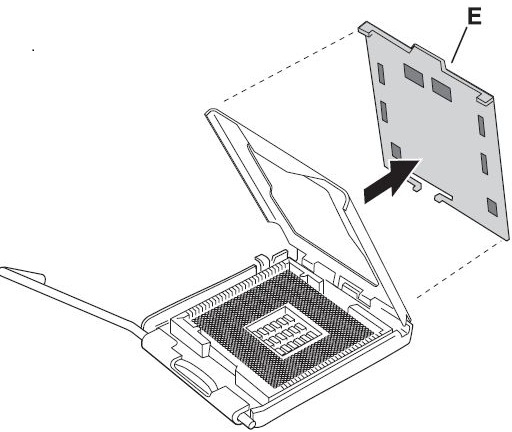
\includegraphics[scale=0.5]{./intelsocket.jpeg}
			\caption{}
			\label{fig.intelsocket}
		\end{subfigure}
		\begin{subfigure}[t]{0.45\textwidth}
			\centering
			{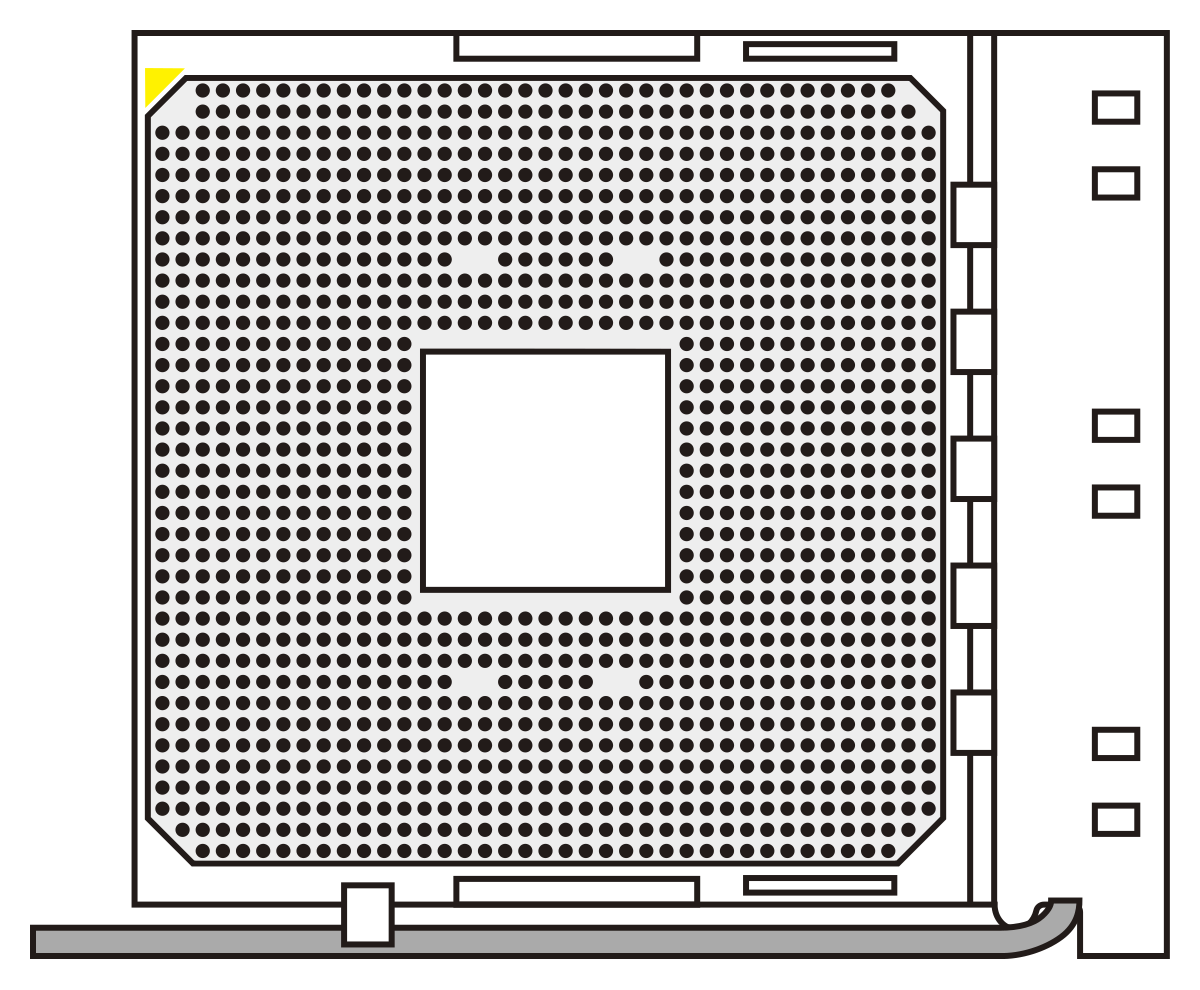
\includegraphics[scale=0.1]{./amdsocket.png}}
			\caption{}
			\label{fig.amdsocket}
			\end{subfigure}	
		\caption{(a) Socket para CPU's Intel, imagem de intel.com.br ; (b) Socket para CPU's AMD, imagem de wikipedia.org }
		\label{fig.sockets}
	\end{figure}	
	
	\item \textbf{Chipset:} Tal como uma motherboard determina diversos elementos e caracterisitcas de um PC, também o chipset determina o tipo de motherboard que temos. O chipset é um conjunto de chips electónicos que controlam não só os nossos componetes e periféricos, como também a compatibilidade entre a nossa Motherboard e os componentes referidos como: \ac{cpu}, \ac{ram}, \ac{gpu}, tipos de \ac{uad}, possibilidade de \textit{overclock}, etc... Cada chipset tem caracteristicas diferentes, sendo que devemos \text{sempre} verificar com os fabricantes do \ac{cpu} escohido, quais os chipsets que o aceitam e , se o nosso processador assim o permitir também, quais desses chipsets permitem \textit{overclock}. 

	\begin{figure}[H]
		\centering
		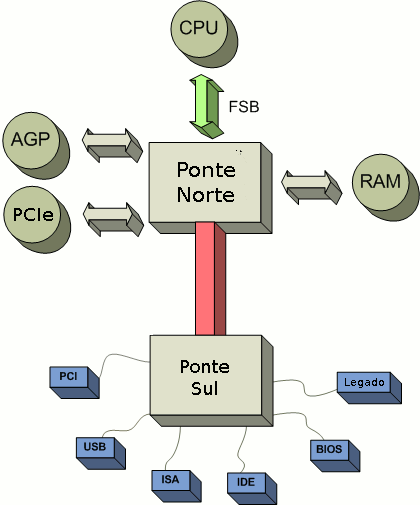
\includegraphics[width=7cm]{./chipsetchart.png}
		\caption{Diagrama simplista de um Chipset , \\ \textsl{imagem de wikipedia.org}}
		\label{fig.cabeçasparafusos}
	\end{figure} 
	
	
	\item \textbf{Tamanho:} O tamanho da nossa motherboard define o tamanho final do nosso PC. Contudo é importante saber que, regra geral: quanto menor uma motherboard menos slots de expanção ela terá, e quanto maior ela for mais slots terá, contudo também será mais cara. \\
	Existem vários tamanhos disponíveis sendo os mais comuns os seguintes:
	
	\begin{itemize}
	\item Extended-ATX - \small mais larga que ATX
	\item Standard-ATX - \small mais comprida que Micro-ATX
	\item Micro-ATX - \small mais comprida e larga que mini-ITX
	\item Mini-ITX - \small modelo mais pequeno
	\end{itemize}	
	
	\begin{figure}[H]
		\centering
		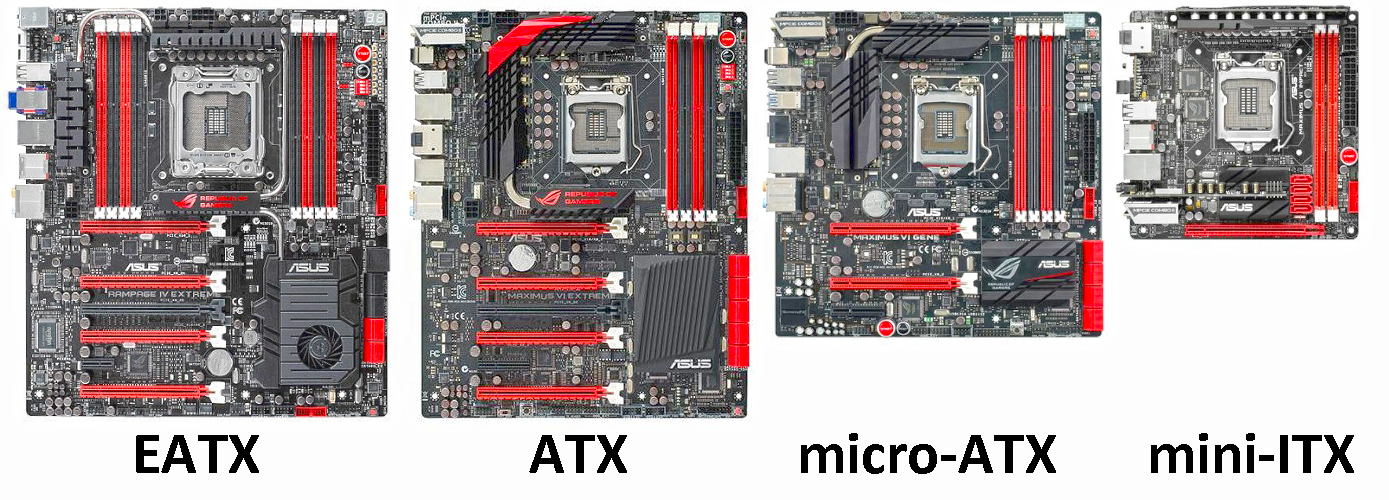
\includegraphics[width=10cm]{./tamanhosMB.png}
		\caption{Exemplares de Tamanhos mais comuns , \\ \textsl{imagem de forum.overclock3d.net}}
		\label{fig.cabeçasparafusos}
	\end{figure} 
	
	\item \textbf{Slots:} Slots são ranhuras presentes na nossa motherboard que permitem o encaixe dos diversos componentes internos. Existem slots para \ac{ram} e slots PCI-E e PCI para placas gráficas e placas de expansão (por exemplo, expansão de número de Portas USB).
	
	\begin{figure}[H]
		\centering
		\begin{subfigure}[t]{0.45\textwidth}
			\centering
			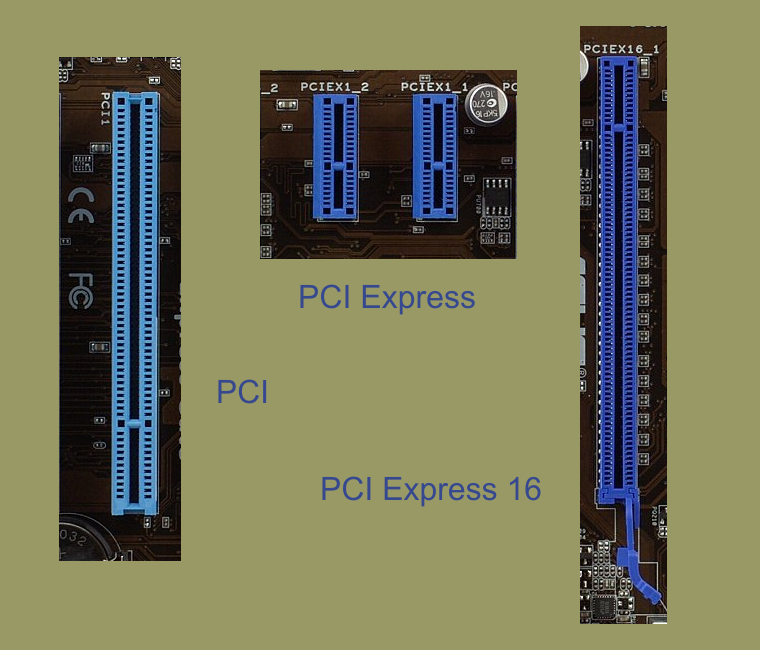
\includegraphics[scale=0.2]{./PCIslots.png}
			\caption{}
			\label{fig.pcislots}
		\end{subfigure}
		\begin{subfigure}[t]{0.45\textwidth}
			\centering
			{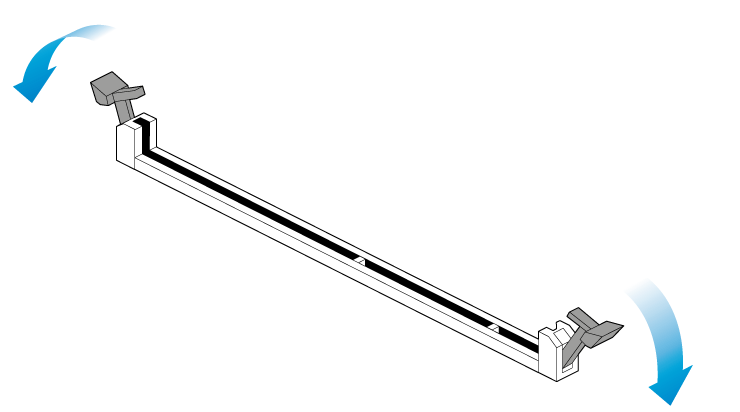
\includegraphics[scale=0.3]{./ramslot.png}}
			\caption{}
			\label{fig.ramslots}
			\end{subfigure}	
		\caption{(a) PCI Slots para gŕafica e placas de expansão, imagem de pt.wikipedia.org  ; (b) Slot de memória RAM, imagem de seagate.com}
		\label{fig.slots}
	\end{figure}	
	
	\item \textbf{Portas I/O:} As portas I/O (ie.: portas de entrada e saida) são, básicamente, as entradas USB, PS2, VGA, HDMI, (etc...) que estão presentes na nossa motherboard nativamente. É importnate termos em atenção o número de portas que dispomos pois são estas que irão conectar todos os nossos periféricos, sendo inconveniente ter mais periféricos que portas disponíveis.
	
	\begin{figure}[H]
		\centering
		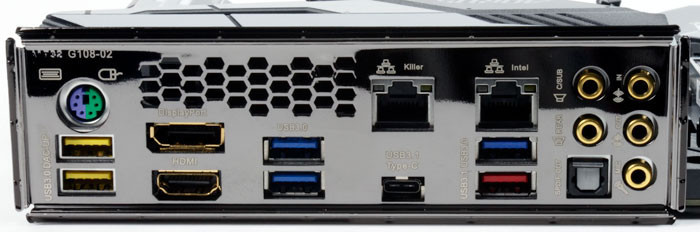
\includegraphics[width=15cm]{./portasIO.jpeg}
		\caption{Exemplar de portas I/O de uma Motherboard , \\ \textsl{imagem de pcmag.com}}
		\label{fig.cabeçasparafusos}
	\end{figure} 
	
	\item \textbf{Headers:} Headers, são pequenos pinos presentes (geralmente) na parte inferior da motheboard que servem para conectar dispositivos do painel frontal da caixa de PC que temos ou vamos adquirir. Estes dispositivos incluem:

	\begin{itemize}
	\item Botão do Power
	\item Botão Reset
	\item Portas USB 2.0 frontais
	\item Portas USB 3.0 e 3.1 frontais (cujos headers são diferentes dos USB 2.0)
	\item Sound jacks 3.5mm frontais para conectar fones e microfones
	\item etc...
	\end{itemize}
	
	\begin{figure}[H]
		\centering
		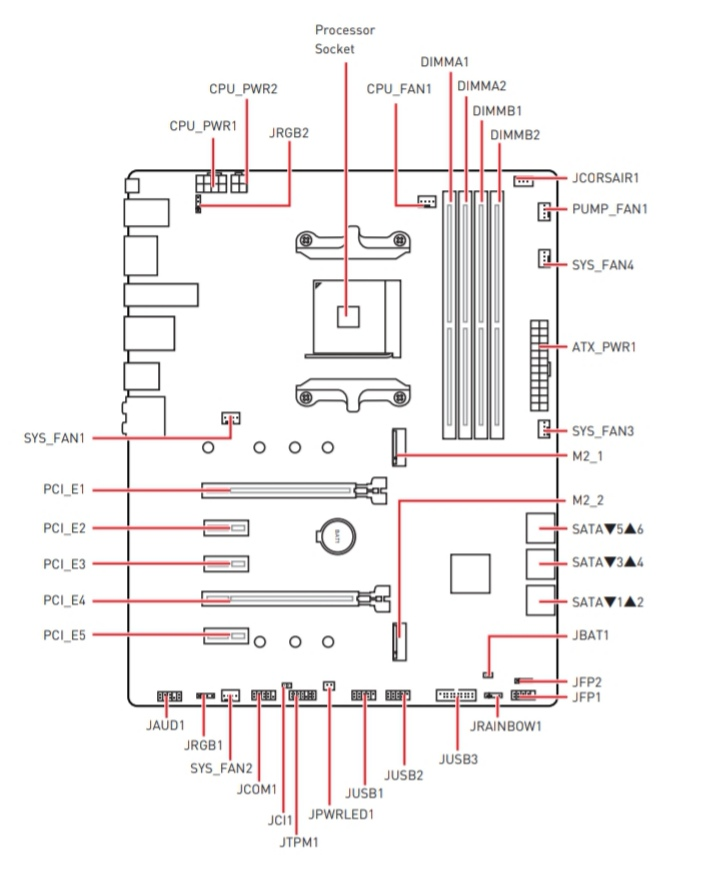
\includegraphics[width=10cm]{./layoutMB.jpeg}
		\caption{Layout exemplare de Motherboard contodas as caracteristica até agora referidas. De notar os Headers JUSB2, JUSB3, JFP1, JAUD1 , \\ \textsl{imagem de forums.tomshardware.com}}
		\label{fig.cabeçasparafusos}
	\end{figure} 
	
\textsl{Nota: Geralmente uma motherboard comum vem sempre com pelo menos 1 header para painel frontal, 1 header para USB 2.0 e 1 header para ligações de audio Jack 3.5mm.}
\end{enumerate}

	\textbf{Dica:} Comprar uma motherboard cara só para ter Wi-fi incorporado, luzes RGB, e outras características "extra" sendo que não vamos usa-las é, essencialmente, um desperdicio de dinheiro que podemos investir noutras peças mais importantes.
	
%########################################################	
%########################################################	
%CAPÍTULO 4: PROCESSADOR
\chapter{Processador}
\lhead{Processador}
\label{chap.cpu}
A unidade central de processamento ou CPU(Central Processing Unit), também conhecido como processador, é a parte de um sistema computacional, que realiza as instruções de um programa de computador, para executar a aritmética básica, lógica, e a entrada e saída de dados. Isto é,realiza operações lógicas,calculos e processamento de dados.\\
A velocidade com que os programas de software operaram é muito dependente de quão poderoso o processador é, por isso é importante ter o tipo certo para as tarefas que deseja realizar. Os dois principais fabricantes de CPU são a Intel e a AMD, cada um com os seus tipos de processadores.\\

A unidade básica de um CPU é divida entre três partes principais:
\begin{itemize}
\item Unidade Lógica e Aritmética (ULA ou ALU): A encarregada de executar as quatro operações básicas (adição, subtração, multiplicação e divisão) e também operações lógicas de álgebra booleana (IF,AND e OR).
\item Unidade de Controle (UC): Responsável por extrair dados da memória,decodificá-los e executá-los, consultando a ULA quando necessários.
\item Registradores: Unidades de memória do CPU, as mais rápidas e consequentemente, as mais caras da sua categoria, sendo reservadas ao uso apenas em CPU, que dependem de velocidades de acesso altas.\\
\end{itemize}
Hoje em dia temos processadores com vários nucleos(dual-core,quad-core,octa-core,hexa-core) que são reponsáveis por dividir as tarefas entre si, ou seja, permitem trabalhar num ambiente multitarefa. Quando havia procesasadores de um só núcleo e eram expostos a uma grande quantidade de tarefas, o seu desempenho baixava, demorando assim bastante tempo para serem processadas. Em processadores com vários núcleos o sistema operacional trata cada um desses núcleos como um processador diferente.\\
Na maioria dos casos, cada unidade possui o seu própio cache e pode processar várias instruções quase simultaneamente.








%########################################################	
%########################################################	
%CAPÍTULO 5: SISTEMAS DE REFRIGERAÇÃO

\chapter{Sistemas de Refrigeração}
\lhead{Sistemas de Refrigeração}
\label{chap.refrigeração}
O sistem de refrigeração de um computador, também conhecido por Cooler, é o componente que tem a função de arrefecer o \ac{cpu} ou \ac{gpu}. O objetivo é evitar o sobreaquecimento termico que estes componentes produzem e consequentemente evitar o (\textit{"shutdown"}) do equipamento ou mesmo a avaria dos componentes em questão.
Existem, essencialmente 4 tipos de \ac{cpu} e {GPU} cooler 

\begin{itemize}
\item \textbf{CPU \ac{oem} Air-Cooler:} é um sistema simples que vem de stock na compra de um qualquer novo CPU (salvo raras excepções "boxless"/sem caixa). É composto por um dissipador de zinco e uam ventoinha simples. Na generalidade estes CPU coolers fazem um trabalho aceitável para sistemas simples onde não se pretende executar uma carga muito grande do programas, contudo existem soluções melhores, mas mais dispendiosas. 


\begin{figure}[H]
		\centering
		\begin{subfigure}[t]{0.45\textwidth}
			\centering
			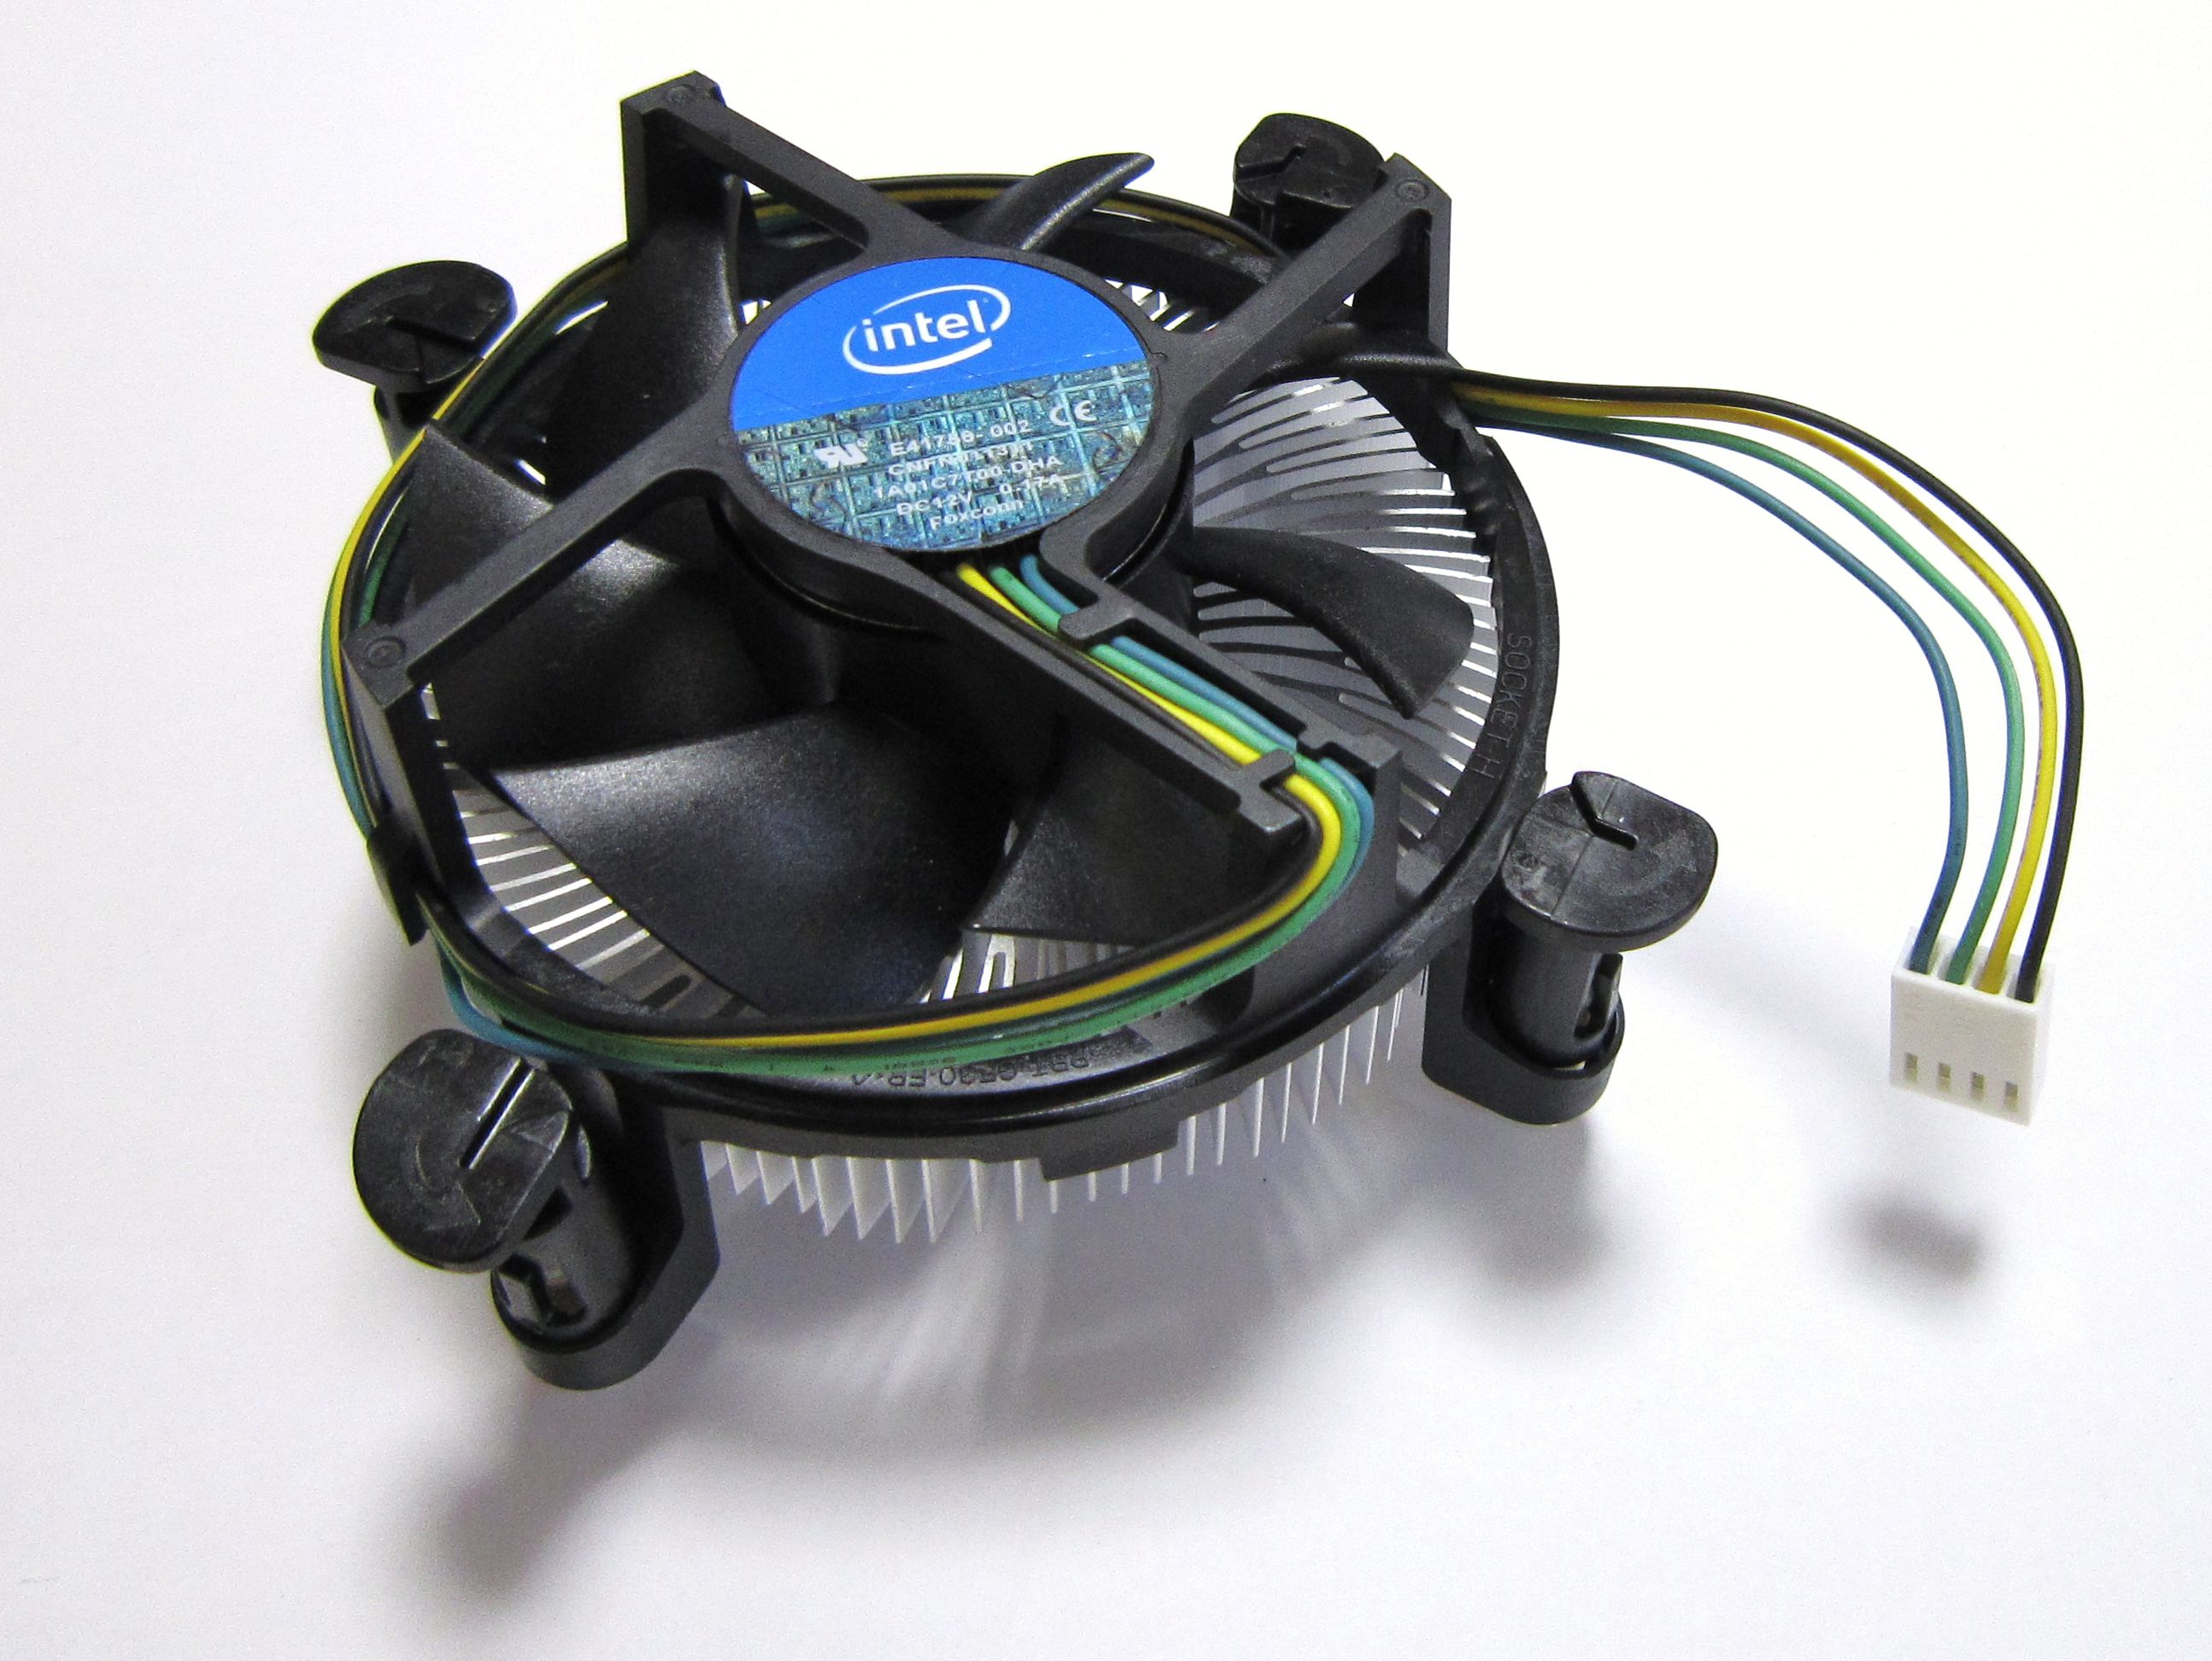
\includegraphics[scale=0.1]{./oemintel.jpeg}
			\caption{}
			\label{fig.oemintel}
		\end{subfigure}
		\begin{subfigure}[t]{0.45\textwidth}
			\centering
			\raisebox{0.8cm}{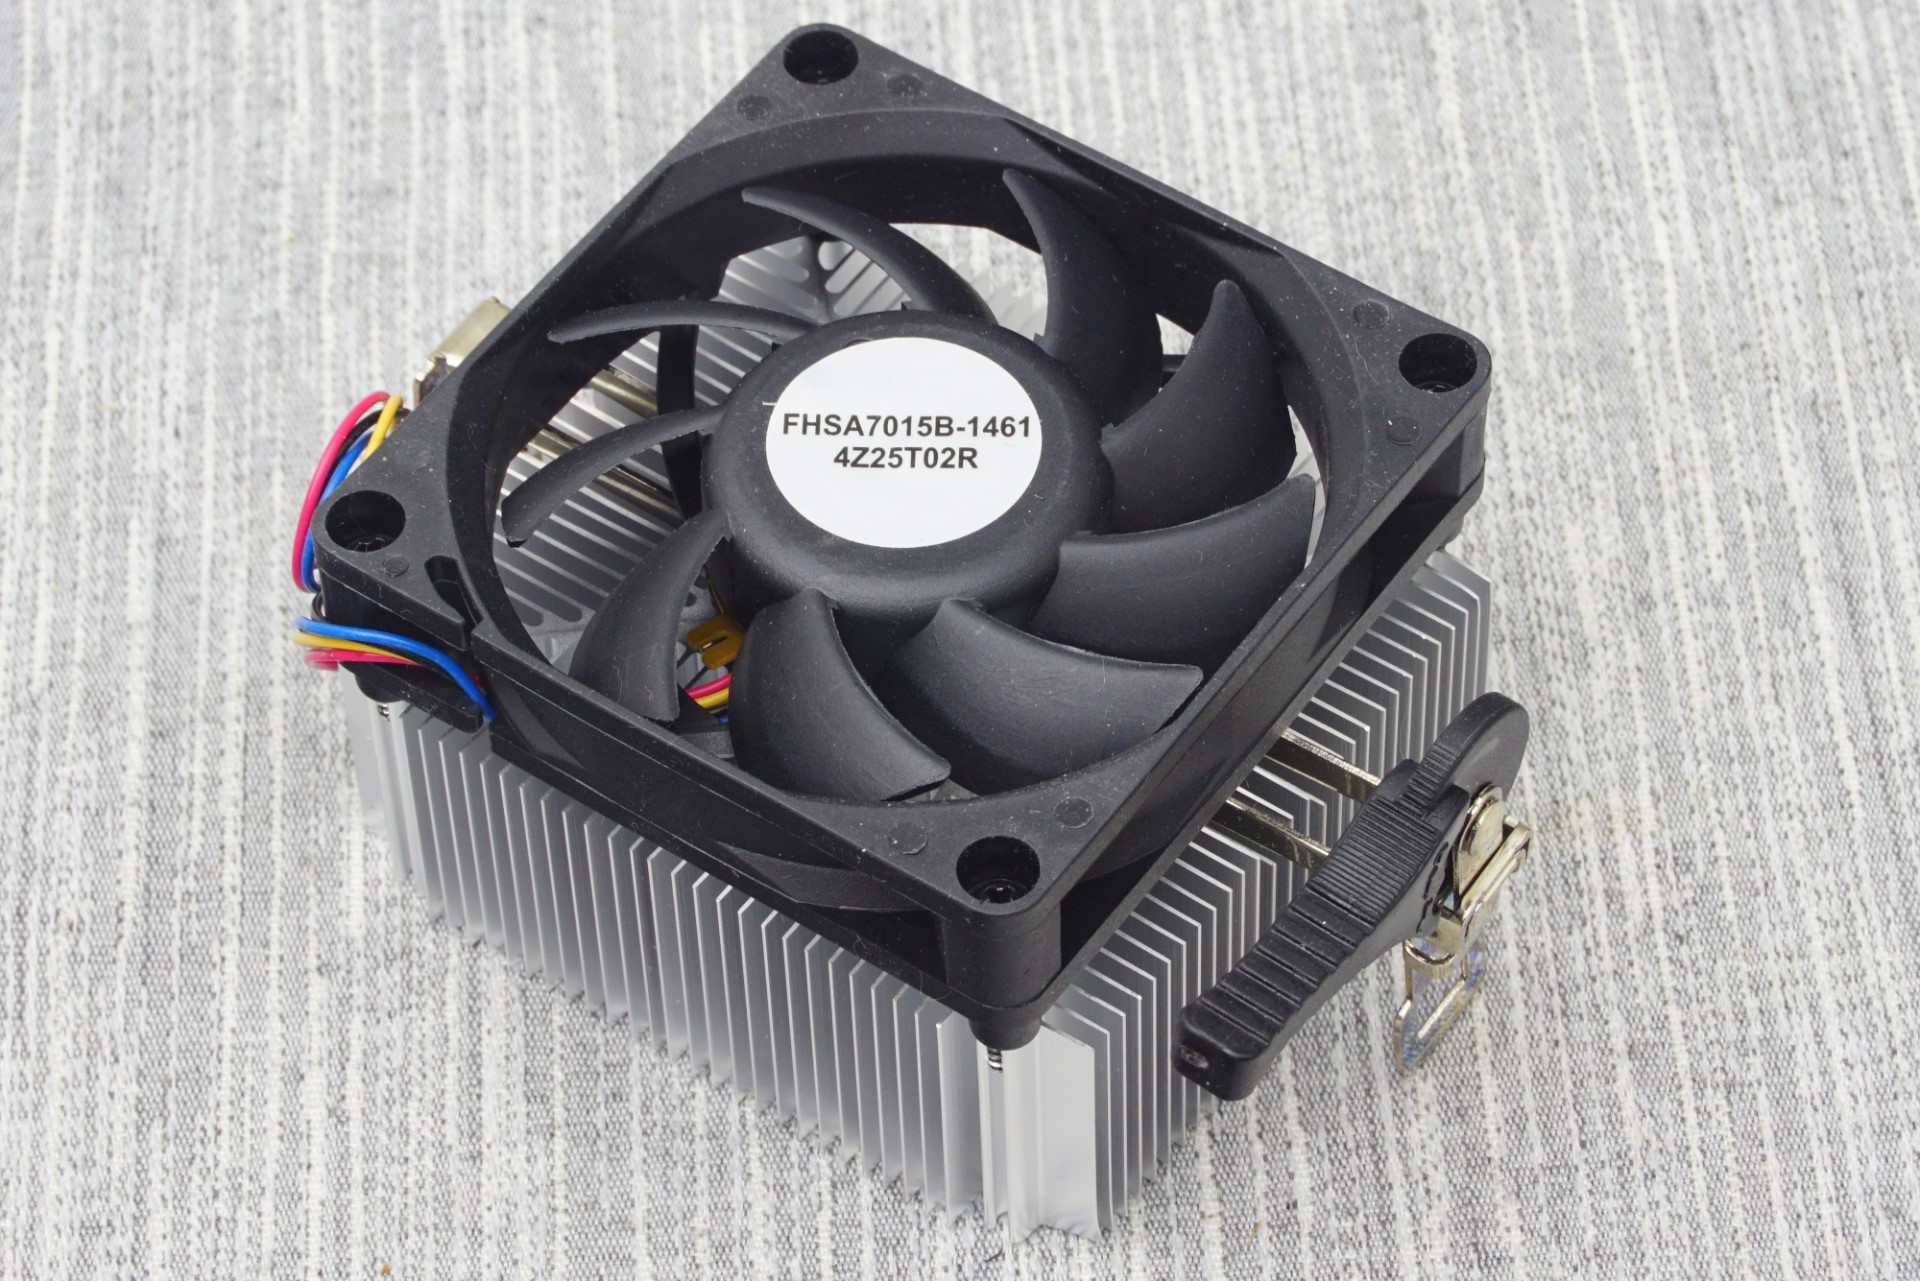
\includegraphics[scale=1]{./oemamd.jpeg}}
			\caption{}
			\label{fig.oemamd}
			\end{subfigure}	
		\caption{(a) OEM Cooler Intel ; (b) OEM Cooler AMD \\ imagens de anandtech.com }
		\label{fig.oemcoolers}
	\end{figure}

	\item \textbf{Air-Cooler com  Heatpipes:} composto por um ventilador plástico polimérico e um dissipador de zinco acoplado com heat pipes de cobre é um sistema de refrigeração muito eficiente e de fácil assemblagem, sendo a escolha ideal para quem quer um sistema de refrigeração robusto e barato. Este tipo de coolers podem ser \ac{oem} em \ac{gpu} e são geralmente adquiridos à parte para \ac{cpu} salvo algumas excelpções (ex.: AMD Ryzen Series).

	\item \textbf{Water-Cooler \ac{aio}:}  Sistema com maior eficiência e maior complexidade que o air-cooler. Utilizados em equipamentos de alta capacidade de processamento, o seu conjunto é composto por uma bomba integrada, um dissipador,um radiador, magueiras e um fluido como refrigerante. No caso dos Water-Coolers \ac{aio} são coolers que já vêm assemblados de fábrica necessitando apenas de ser montados no interior do PC. 
\end{itemize}

\textbf{Nota:} Existe ainda uma solução mais complexa. Um Water-Cooler Costum, ie.: que vem às peças (desmontado) ou são adquiridas peças de diferentes fabricantes para produzir um modelo costumizado. Esta última solução é recomendada apenas para utilizadores experientes, pois existem riscos inerentes à mesma: fugas de liquido, bolhas de àr, etc... \\

\begin{center}
\textbf{Porque é que o Water-cooling é o sistema mais eficiênte?}	\\
O líquido apresenta em comparação com o ar uma maior capacidade de condutividade térmica, o que representa uma clara vantagem versus o Air-Cooler. Isso significa que o líquido é capaz de mover calor de uma forma mais rápida que o ar caso do air-cooling,trazendo assim mais efetividade na sua eliminação.
\end{center}

%########################################################	
%########################################################	
%CAPÍTULO 6: PLACAS GRÁFICAS
\chapter{Placas Gráficas}
\lhead{Placas Gráficas}
\label{chap.gráficas}
  A placa gráfica, é um componente de um computador que envia sinais para o ecrã, de forma a que possam ser apresentadas imagens ao utilizador.Normalmente possui memória com capacidade medida em Byte. É responsável por gberar e renderizar gráficos tanto 2D como 3D.
  Originalmente, as placas gráficas eram dispositivos simples, que se limitavam a mostrar o conteúdo da memória de vídeo no monitor. A resolução máxima suportada pela placa gráfica era limitada pela quantidade de memória de vídeo. Na época, memória era algo caro, e desta forma as placas vinham apenas com 1MB ou 2MB. As placas de 1MB permitiam usar no máximo 800 x 600 com 16 bits de cor, ou 1024 x 768 com 256 cores.
  Em seguida, as placas poassaram a suportar recursosde aceleração,que permitem fazer coisas como mover janelas ou procesasar arquivos de vídeo de forma a aliviar o processador principal.\\
Finalmente ,as placas deram um passo final, passando a suportar recursos 3D. Imagens em três dimensões são formadas por polígonos, que formas geométricas como triângulos e retângulos em diversos formatos. Qualquer objeto em um jogo 3D é formado por um grande número destes polígonos com uma cor e tamanho específico.\\  


\section{On-Board}
  Em computadores mais baratos,as placas gráficas estão incorporadas na motherboard, que são as mais comuns. Por não possuírem memória dedicada,utilizam a memória RAM do sistema.
  De uma forma geral, as placas gráficas on-board (pelo menos os modelos que dispõem de drivers adequados) atuais atendem às tarefas do dia-a-dia. Elas também permitem jogar os jogos mais antigos.Placas mais sofisticadas são resevadas a quem faz questão de jogar os jogos mais recentes com uma boa qualidade
\section{Off-Board}
  Já em compoutadores mais sofisticados, a placa gráfica é separada da motherboard. Trata-se de um processador capaz de gerar imagens e efeitos visuais tridimensionais e acelerar os bidimensionais, diminuindo o trabalho do CPU e gerando um resultado final melhor e mais rápido. Esse processador utiliza uma linguagem própia para a descrição das imagens tridimensionais, assim sendo interpretado,executado e posteriormente gerar o resultado final,que é a imagem vista pelo observador. Esse resultado final normalmente é medido considerando o número de vezes por segundo que o computador consegue redesenhar uma cena,cuja a medida é o FPS (Frames Per Second).
  As placas off-board 3D tambvém incluem uma quantidade generosa de memória de vídeo (512 MB, 768 MB, 1 GB, 2 GB, 8 GB, mais nos modelos mais recentes). O GPU (o chipset da placa) é também mais poderoso, de forma que as duas combinam para oferecer um altíssimo desempenho.\\
  Com a evolução do 4D, os vídeos passaram a utilizar gráficos mais elaborados, explorando os recursos das placas recentes.  









%########################################################	
%########################################################	
%CAPÍTULO 7: MEMÓRIAS RAM
\chapter{Memória RAM}
\lhead{Memória RAM}
\label{chap.ram}
A memória RAM(Random Acess Memory - Memória de Acesso aleatório) é um hardware de armazenamento aleatório e volátil de memória. Isto significa que esta peça armazena dados de programas em execução enquanto o computador está ligado.\\
A memória RAM é de acesso rápido, ou seja, é essecial para acompanhar a velocidade do processador. Este tipo de memória recebe informações do HDD ou SSD, e armazena-as temporariamente, disponibilizando este conteúdo ao processador.Seria muito mais lenta a execução caso o processador tivesse de procurar os dados diretamente do HHd ou SSD.\\
A produção deste documento de texto é um exemplo prático para explicar a função da RAM. Enquanto o autor está a escrever e editando texto, os dados ficam na memória RAM. Após o documento ser gravado num diretório, passa a ser armazenado no HHD ou no SSD.  

\section{Diferenças entre os tipos de memória}
\begin{itemize}
\item DDR RAM: Lançada em 2000.Funcionava a 2.5V e 2.6V,tendo uma capacidade máxima de 128MB a 266 MT/s(100-200 MHz)
\item DDR2 RAM:Lançada em 2004. Apresentando esta 28\% menos voltagem(1.8V) do que a DDR. A capacidade máxima aumentou para o dobro,assim como a velocidade máxima, alcançando 533 MHz.   
\item DDR3 RAM:Esta foi lançada em 2007,tornando-se revolucionária uma vez que foi emplementado XMP(Extreme Memory Profiles),dando a opção ao utilizador de dar overclock á RAM, atingindo a memória desta forma velocidades maiores. Funcionava a 1.5V e 1.65V com uma frequência de 1066MHz.
\item DDR4 RAM:A voltagem, em relação á anterior baixou para 1.05V e 1.2V. Nesta última a velocidade aumentou consideravelmente,começando a uma frequÊncia de 2133MHZ.
\end{itemize}
Num passado recente esta tecnologia tem evoluído exponencialmente, sendo de esperar que a DDR 4 seja ultrapassada e surja uma nova com velociades superiores.

%########################################################	
%########################################################	
%CAPÍTULO 8: MEMÓRIA INTERNA HDD E SSD
\chapter{Memória Interna de Armazenamento}
\lhead{Memória Interna de Armazenamento}
\label{chap.armazenamento}
\section{HDD}
  HDD(Hard Disk Drive), é parte do computador onde são armazenados os dados. O disco rígido é uma memória não volátil, ou seja, as informações não são perdidas quando o computador é desligado, sendo considerado o principal meio de armazenamento de uma grande quantidade de dados. É um sistema necessário para se ter um meio de executar novamente programas e carregar ficheiros contendo os dados inseridos anteriormente quando ligamos quando ligamos o computador.\\
\section{SSD}
  SSD(Solid-State Drive),é também outro mecanismo de armazenar dados. São tipicamente , construídos em torno de um circuito integrado semicondutor, responsável pelo armazenamento, ao contrário dos sistemas magnéticos (como os HDDs). Os despositivos utilizam memŕia flash (tecnologia semelhante ás utilizadas em cartões de memória)
\subsection{Vantagens}
\begin{itemize}
\item Eliminação de partes móveis eletromecânicas, reduzindo vibrações, tornando-os completamente silenciosos.
\item Por não possuírem partes móveis,são muito mais resistentes que os HDDs comuns contra choques físicos.
\item Menos pesado em relação aos discos rígidos, mesmo os mais portáteis.
\item Consumo reduzido de energia. 
\item Possibilidade de trabalhar em temperaturas maiores (cerca de 70 graus Celsius) 
\item Apresenta velocidades de gravação e de leitura,apresentando até 4500 MB/s na gravação e até 5000 MB/s nas operações de leitura.
\end{itemize}
\subsection{Desvantagens} 
\begin{itemize}
\item Custo mais elevado.
\item Capacidade de armazenamento inferior aos discos rígidos.
\end{itemize}  






%########################################################	
%########################################################	
%CAPÍTULO 9: FONTES DE ALIMENTAÇÃO
\chapter{Fontes de Alimentação}
\lhead{Fontes de Alimentação}
\label{chap.psu}

A \ac{psu} , (do inglês: Power Supply Unit) é um componente interno que distribui corrente electrica por todos os restantes componentes, permitindo assim ao computador funcionar. Contudo, muitas vezes são esquecidas ou menospresadas, o que é um erro. A \ac{psu} executa duas funções fundamentais na alimentação electrica do PC:

	\begin{enumerate}
	\item Distribui e mantém a corrente elétrica estável
	\item Protege o equipamento de picos de tensão elétrica
	\end{enumerate}
	
Uma \ac{psu} deve ser escolhida por forma a \textsf{"aguentar"} os compoentes internos, ie., a fonte deve alimentar o PC de tal maneira que o sistema não consuma mais potencia do que aquela que é destribuida pela fonte. Existem assim, características importantes na escolha de uma boa \ac{psu} nomeadamente:
	\begin{itemize}
	\item \textbf{Potência:} Medida em \ac{w} (unidade de potência no \ac{si} ), é uma característica fundamental no processo de escolha. Esta medida determina quanta potência a \ac{psu} pode debitar no seu limite de trabalho. Assim, é sempre conveniente escolher uma fonte com potência superior à potencia consumida pelo computador. Existem diversas formas de calcular esta potencia consumida do PC, contudo fazemos referencia aos seguintes websites de marcas fidignas para fazer os calculos de forma simplificada: 
		\begin{itemize}
		\item $https://www.asus.com/microsite/power_supply_calculator/$
		\item $https://www.coolermaster.com/power-supply-calculator/$
		\item $https://seasonic.com/wattage-calculator$
		\end{itemize}
	Basta inserir o Hardware do PC e o website apresenta uma estimativa fiável para a potência necessária para a \ac{psu} a assemblar no equipamento.
	\item \textbf{\ac{pfc} :} esta característica permite à \ac{psu} que funcione com a máxima eficiencia possível. Assim existem dois tipos distintos de \ac{pfc}:
		\begin{itemize}
		\item{\ac{pfc} Passivo:} este tipo de \ac{pfc} é o mais comum existente em fontes de alimentação baratas de baixa gama. Não usa todo o potencial de energia, sendo a sua eficiencia inferior e assim, não é tão confiável.
		\item{\ac{pfc} Activo:} este é o tipo de \ac{pfc} que é mais recomendado, já que fornece energia de uma forma mais eficiente usando um circuito para corrigir o fator de potência, é capaz de produzir (teóricamente) um fator de potência de cerca de 95~\%. Também tem harmônicos totais diminuidos e é capaz de corrigir automáticamente a tensão de entrada AC.
		\end{itemize}
	\item \textbf{\ac{80+} :} este certificado criado em 2004 pela \textit{Ecos Consulting}, certifica produtos que tem mais que 80~\% de eficiência energética. Assim existem subcategorias deste certificado que ajudam o utilizador/comprador a ter uma noção do quanto eficiente é a \ac{psu} que pretende adquirir:
	
\begin{table}[H]
    \centering
    \caption{Eficiencia \acf{80+} , 230 V EU interno não redundante}
    \begin{tabular}{|c|c|c|c|c|c|c|}\hline
        Percentagem de carga nominal & Standard & Bronze & Silver & Gold & Platinum & Titanium  \\ 
        \hline
        10~\% &       &       &       &       &       & 90~\% \\
	    20~\% & 82~\% & 85~\% & 87~\% & 90~\% & 92~\% & 94~\% \\
	    50~\% & 85~\% & 88~\% & 90~\% & 92~\% & 94~\% & 96~\% \\
	   100~\% & 82~\% & 85~\% & 87~\% & 89~\% & 90~\% & 94~\% \\
	  \hline
    \end{tabular}
    \label{tab.80plus}
\end{table}		
	
	\begin{figure}[H]
	\centering
	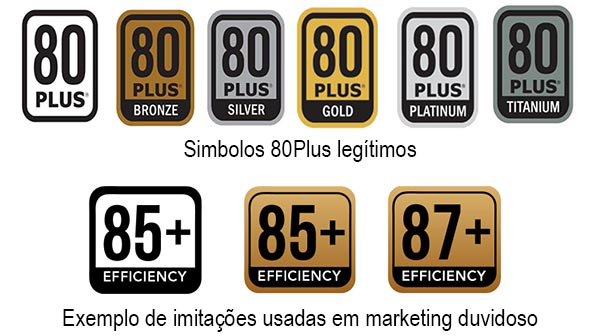
\includegraphics[width=10cm]{./80plus.jpeg}
	\caption{Selos Certificado 80 Plus comparados com selos de certificados de carís duvidoso;\\ \textsl{imagem de portal.zwame.pt}}
	\label{fig.80plus}
	\end{figure} 
	\item \textbf{Marca :} as marcas de \ac{psu} são importantes, pois existem algumas que criam os seus próprios selos \ac{80+} de carís duvidoso. Assim recomendamos escolher uma marca de renome cujo selo seja efectivamente \ac{80+} e não 85+ ou qualquer outro valor. Algumas marcas recomendadas são:
		\begin{itemize}
		\item Corsair
		\item Gigabyte
		\item EVGA
		\item Cooler Master
		\item ASUS
		\item NZXT
		\end{itemize}
		
	\item \textbf{Cabos e Ligações :} Para finalizar, é necessário verificarmos se o número de cabos e respectivas ligações são as adequadas ao nosso sistema. Neste caso em especial, quantos mais cabos melhor, pois temos maior versatibilidade para \textit{upgrades} futuros. Contudo para evitar um grande aglomerado de cabos no interior do PC recomendamos a quisição de uma \ac{psu} semi ou full-moderal (ie.: fontes de alimentação com cabos removíveis em caso de não utilização).
	\end{itemize}

%########################################################	
%########################################################	
%CAPÍTULO 10: CAIXAS DE PC:

\chapter{Caixas de PC} 
\lhead{Caixas de PCs}
\label{chap.chassi}
 De uma forma geral,uma caixa de um PC incluirá quatro ou cinco compartimentos (bays) para unidades de discos, uma fonte de alimentação com os respetivos cabos para alimentar as diversas unidades a instalar,um botão de reinicialização (reset), um interrupetor (power switch), uma chave de segurança para o teclado (key lock) e um conjunto de indicadores luminosos. Mas independente da estética ou da maior ou menor capacidade de expansão, uma caixa deverá albergar em boas condições técnicas uma motherboard, uma fonte de alimentação e um conjunto de periféricos de armazenamento de informação . E as boas condições técnicas começam pela garantia de um bom fluxo de ar, que permita o arrefecimento adequado dos componentes mais criticos (CPU e processador gráfico,tipicamente), passam por uma estrutura rígida e geometricamente bem concebida, que confira ao conjunto uma rebustez adequada , e acabam no nível de eficiência que conferem,quer pela acessibilidade,quer pela segurança (hoje em dia cada vez mais relevante). Todos estes fatores devem ser levados em conta aquando a escolha da caixa correta, em função da utilização.

 Para classificar os tipos de caixas existentes , é vulgar distingui-las pelo seu formato:
\begin{itemize}

\item Desktop: existem com dois perfis,nomeadamente delgadas (slim) e altas (tall). As primeiras não têm altura para uma placa de extensão, levando, para o efeito,uma placa extra na vertical,com dois ou três conectores,para aí inserrir horizontalmente as referidas placas de expansão. Este excesso de contactos revela-se um problema, e isto para além da natural limitação relativa ao número de compartimentos resultante da sua pequena dimensão. As caixas tall não evidenciam qualquer tipo de problema, facultandol mesmo muitas vezes a melhor acessibilidade aos diversos componentes. 

\item Tower: existe,habitualmente, em três tamanhos, mini, mid, full. As mais divulgadas são as mini tower e as full tower, mas é possível encontrar, para aplicações específicas (particularmente servidores)
\end{itemize}

Finalmente, as chamadas caixas de "PC Industrial". Estas caixas caracterizam-se,habitualmente , por um nível de robustez adicional, o que se justifica dada a frequente agressividade do ambiente em que essas máquinas são utilizadas. Variam muito da forma e na capacidade de expansão, sendo fornecidas ,na maior parte de um equipamento maior (em termos de utilizador final), como por exemplo, uma máquina de jogos eletrónicos. 

%########################################################	
%########################################################	
%CAPÍTULO 11: MONITORES:
\chapter{Monitores}
\lhead{Monitores}
\label{chap.monitores}
Uma vez que na montagem de uma computador é necessário um monitor,seguem-se alguns tipos e as suas características.

\section{Monitores LCD}
\begin{itemize}
	\item Têm um preço económico se forem tamanhos menores que 40" e um preço mais alto ao exceder essa medida.
	\item A resolução é maior que a de um plasma.
	\item Existe uma grande variedade de tamanhos.
	\item Leve, compacto e portátil.
	\item Possui baixa relação de contraste.
	\item O ângulo de visão é inferior ao dos monitores de plasma.
\end{itemize}

\subsection{Monitores de Plasma}
\begin{itemize}
	\item Os mais económicos possuem tamanhos acima de 40".
	\item Maior ângulo de visão em relação ao LCD.
	\item Melhor relação de contraste , isto significa, uma melhor reprodução da cor preta. 
	\item Resolução mais baixa em relação aos LCDs.
	\item É possível observar reflexos na tela.
	\item Maior consumo de energia.
\end{itemize}

\subsection{Monitores LED}
\begin{itemize}
	\item Boa relação de contraste.
	\item Telas finas, de 2.5 cm.
	\item Baixo consumo de energia.
	\item Possuem a mesma resolução nativa de 1280x720 pixels que as LCDs. 
	\item Possuem um preço mais alto.
	\item Têm poucos tamanhos dispoíveis.
	\item Longa duração.
\end{itemize}

Para fãs do gaming na altura da escolha de um monitor aconselha-se a escolher monitores com a tecnologia IPS (In-Plane Switching). Duas das suas principais características dessa tecnologia é o seu alto ângulo de visão,chegando a 178 graus e a alta taxa de atualização de imagens, tipicamente 240 Hz, o que torna a transição de imagens mais suave, sendo ideal tanto em filmes como em jogos.Para comparação , um monitor convencional  tem uma área de visao de 160 graus e taxa de atualização de 60 Hz.

\subsection{Saúde Ocular} 
Mesmo não estando este tema diretamente relacionado com o intuito do trabalho(e portanto, é feito só um pequeno alerta)  é importante alertar sobre os danos que a nossa visão poderá sofrer. Estando cada vez o Ser Humano mais ligado aos computadores, é essencial moderar a sua utilização.

Estudos indicam que mais de 50\% das pessoas que trabalham em frente a um ecrã de um computador sofre do que se chama de cansaço visual digital. Isso implica cansaço, olhos secos, irritados e com comichão, além de dores de cabeça. Isto está relacionado com o excesso de exposiçao a luz intensa emitida por aparelhos digitais. Quanto melhor a qualiddade e menos brilho maior sõo as hipóteses de não ter estes simtomas. 
 
%########################################################	
%########################################################	
%ACRÓNIMOS:

\chapter*{Acrónimos}
\begin{acronym}
\acro{ua}[UA]{Universidade de Aveiro}
\acro{miect}[MIECT]{Mestrado Integrado em Engenharia de Computadores e Telemática}
\acro{jv}[JV]{Autor: \pautor , \numpautor - }
\acro{pm}[PM]{Autor: \sautor , \numsautor - }
\acro{cpu}[CPU]{Processador}
\acro{ram}[RAM]{Memória de Acesso Aleatório}
\acro{uad}[UAD]{Unidade de Armazenamento de Dados}
\acro{hdd}[HDD]{Unidade de Disco Rígido}
\acro{ssd}[SSD]{Unidade de Disco Sólido}
\acro{oem}[OEM]{Fabricante Original do Equipamento}
\acro{aio}[AIO]{All-in-One}
\acro{psu}[PSU]{Fonte de alimentação}
\acro{w}[W]{Watt's}
\acro{si}[SI]{Sistema Internacional de Unidades}
\acro{pfc}[PFC]{Power Factor Correction}
\acro{80+}[80 +]{Certificado 80 Plus}
\acro{gpu}[GPU]{Unidade de Processamento Gráfico}
\end{acronym}

%########################################################	
%########################################################	
%CONTRIBUIÇÕES DE AUTORES:

\chapter*{Contribuições dos Autores}
\ac{jv} \\
\ac{pm} \\
\begin{table}[H]
    \centering
    \caption{Contribuições dos Autores.}
    \begin{tabular}{|c|c|c|c|}\hline
        Contribuição & \ac{jv} & \ac{pm}  \\ 
        \hline
	    Produção Latex & 80~\% & 20~\%    \\
	    Resumo &  & 100~\%  \\
	    Agradecimentos & 100~\% &   \\
        Introdução & 100~\% &    \\
       	Ferramentas e Cuidados Essenciais  & 50~\% &  50~\%    \\
       	Motherboards & 100~\% &  \\
       	Processadores &  & 100~\% \\
        Sistemas de Refrigeração & 50~\%  & 50~\% \\
		Placas Gráficas	&  &  100~\% \\	
		Memória RAM & & 100~\% \\ 
        Memória Interna de Armazenamento & 50~\% & 50~\% \\
        Fontes de Alimentação & 100~\% & \\
        Caixas de PC & & 100~\% \\
        Monitores & & 100~\% \\
        Acrónimos & 100~\% &  \\ 
        Bibliografia & 80~\% & 20~\%   \\
    \hline
    \end{tabular}
    \label{tab.contribuições}
\end{table}	

%########################################################	
%########################################################	
%BIBLIOGRAFIA:

\begin{thebibliography}{9}

\bibitem{ibm} 
André Emonet, Eurico da Fonseca e Paulo Goulão.
\textit{IBM, 50 anos em Portugal}. 
Departamento de Compunicações e Programas Externos da Companhia IBM Portuguesa S.A., 1ª Edição, Portugal, 1988.

\bibitem{thompson}
Thompson, Robert Luis and Thompson, Barbara Fritchman.
\textit{PC Hardware in a Nutshell}.
O'Reilly and Associates Inc , First Edition , October 2000

\bibitem{INEwebsite}
INE: Instituto Nacional de Estatística, Statistics Portugal.
\text{ine.pt, acedido 10/12/2020.}

\bibitem{Wikipedia}
Wikipédia: Enciclopédia livre. 
\text{ pt.wikipedia.org, acedido 18/12/2020.}

\bibitem{Infoduvidas}
Infoduvidas Website.
\text{ sites.google.com/site/infoduvidas1/home, acedido 18/12/2020.}

\bibitem{Wikipedia}
ELGScreen Website.
\text{ elgscreen.com/componentes-do-pc/, acedido 18/12/2020.}


\bibitem{Wikipedia}
Coopervision Website: Live Brightly
\text{ coopervision.pt, acedido 18/12/2020.}

\bibitem{Tomshardware}
Tomshardware Website: Forum and Tech Reviews.
\text{forums.tomshardware.com , acedido 18/12/2020.}

\bibitem{PCmag}
PCMag Website: Tech Reviews Magazine
\text{ pcmag.com, acedido 18/12/2020.}

\bibitem{Zwame}
Zwame Website: Forum.
\text{ portal.zwame.pt, acedido 18/12/2020.}

\bibitem{ASUSwebsite}
ASUS Website. 
\text{ asus.com/pt/, acedido 18/12/2020.}

\bibitem{CMwebsite}
Cooler Master Website: "Make it Yours". 
\text{ coolermaster.com, acedido 19/12/2020.}

\bibitem{AnandTech}
Anandtech Website: Reviews and Guides. 
\text{ anandtech.com.com, acedido 19/12/2020.}


\end{thebibliography}
\end{document}